\documentclass{article}

\usepackage[preprint]{corl_2026}

\usepackage[utf8]{inputenc}
\usepackage[T1]{fontenc}
\usepackage{amsmath,amssymb,bm}
\usepackage{booktabs}
\usepackage{graphicx}
\usepackage{tikz}
\usetikzlibrary{arrows.meta,positioning,calc,fit,backgrounds}
\usepackage{pgfplots}
\pgfplotsset{compat=1.18}
\usepgfplotslibrary{groupplots}
\usepackage{listings}
\usepackage{xcolor}
\usepackage{microtype}
\usepackage{float}

% ---------- notation and helpers shared by both layouts ----------
\newcommand{\code}[1]{\texttt{#1}}
\newcommand{\subl}[1]{{\scriptsize\color{black!60}#1}}
\definecolor{series1}{HTML}{2A78D6}
\definecolor{series2}{HTML}{EB6834}
\definecolor{band}{HTML}{E7EEF1}
\definecolor{codebg}{HTML}{F4F5F4}
\definecolor{stagefill}{HTML}{DFEAEF}
\definecolor{stageline}{HTML}{1F6F8B}
\lstset{
  language=Python,
  commentstyle=\color{black!55}\itshape,
  keywordstyle=\bfseries,
  stringstyle=\color{black!70},
  backgroundcolor=\color{codebg},
  frame=single, framerule=0pt, framesep=3pt,
  columns=fullflexible, keepspaces=true,
  breaklines=true, breakatwhitespace=false, showstringspaces=false,
  numbers=left, numberstyle=\tiny\color{black!45}\ttfamily, numbersep=5pt, stepnumber=1,
  xleftmargin=18pt, xrightmargin=2pt,
  aboveskip=1pt, belowskip=0pt,
  literate={ö}{{\"o}}1 {ä}{{\"a}}1 {·}{{$\cdot$}}1 {—}{{--}}1 {→}{{$\to$}}1,
}
% file header above a listing: path on the left, line range on the right
\newcommand{\snippethead}[2]{\par\noindent{\scriptsize\sffamily\color{black!60}\path{#1}\hfill\mbox{#2}}\par\nopagebreak\vspace{-2pt}}
\newcommand{\snippetelide}{\par\nopagebreak\vspace{-5pt}\noindent{\scriptsize\color{black!45}\ttfamily\hspace{6pt}$\vdots$}\par\nopagebreak\vspace{-6pt}}
\tikzset{
  blk/.style={draw=black!55, rounded corners=2pt, minimum height=8mm, align=center, font=\small, inner sep=3pt, fill=black!4},
  stage/.style={blk, fill=stagefill, draw=stageline, line width=0.8pt},
  sub/.style={font=\scriptsize\color{black!60}},
  arr/.style={-{Latex[length=2mm]}, thick, black!70},
  darr/.style={-{Latex[length=2mm]}, thick, dashed, black!55},
}
% a snippet (header + listing, possibly with elisions). The optional argument is the number of text lines that
% must still fit on the page before the snippet may start, so the header always stays with the first code lines;
% a long listing may then break across pages instead of leaving a large gap at the page bottom.
\newenvironment{snippetbox}[1][8]{\par\addvspace{4pt}\penalty0
  \ifdim\pagegoal=\maxdimen\else
    \ifdim\dimexpr\pagegoal-\pagetotal\relax<#1\baselineskip \newpage\fi
  \fi
  \lstset{aboveskip=1pt, belowskip=0pt}}{\par\addvspace{4pt}}

\lstset{basicstyle=\ttfamily\scriptsize}

% figure and table wrappers: placed exactly where they are referenced (no floating)
\newenvironment{myfigure}{\begin{figure}[H]\centering}{\end{figure}}
\newenvironment{mytable}{\begin{table}[H]\centering}{\end{table}}
\newcommand{\myfigcaption}[2]{\caption{#2}\label{#1}}
\newcommand{\mytabcaption}[2]{\caption{#2}\label{#1}}

\title{Two Simulators, One Controller:\\ The Stage 1 and Stage 2 Training Recipe in OmniReset}

\author{
  Tri Wahyu Guntara\\
  Training notes on the UWLab OmniReset code base\\
}

\raggedbottom

\begin{document}
\maketitle

% Shared body of the two-stage training note. Included by the CoRL-style and the quick-guide-style main.tex.
% Figure/table wrappers (myfigure, mytable, \mycaption) are defined by the including preamble.

This note is a companion to the controller tutorial \emph{From a Desired End-Effector Pose to Joint Torques} in the same folder. That tutorial explains how the relative Cartesian operational-space controller (OSC) turns a policy action into joint torques~\cite{khatib1987unified}. This note explains what happens to those torques afterwards, and how the training recipe is organised around that.

%==============================================================================
\section{The Two Stages at a Glance}
\label{sec:overview}

The OmniReset insertion policy~\cite{omnireset2026} is trained in two stages. Stage~1 trains the policy from scratch in a deliberately forgiving simulator. Stage~2 loads the converged stage~1 checkpoint and continues training while the simulator is gradually made to behave like the physical robot. The controller, the reward, the observations and the network are identical in both stages. What changes is the plant that the controller acts on, together with the gains and the action scale that the controller is given. Figure~\ref{fig:stages} summarises the recipe.

\begin{myfigure}
\resizebox{\linewidth}{!}{%
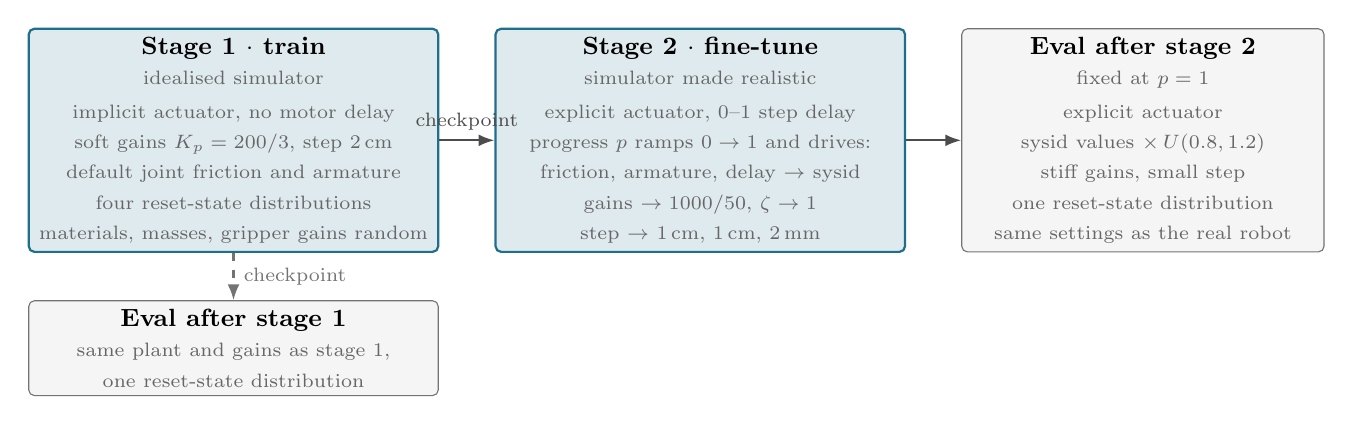
\begin{tikzpicture}[node distance=4mm and 7mm]
  \node[stage, minimum width=52mm] (s1) {\textbf{Stage 1 $\cdot$ train}\\ \subl{idealised simulator}\\[1pt]
    \subl{implicit actuator, no motor delay}\\ \subl{soft gains $K_p=200/3$, step 2\,cm}\\ \subl{default joint friction and armature}\\ \subl{four reset-state distributions}\\ \subl{materials, masses, gripper gains random}};
  \node[stage, right=of s1, minimum width=52mm] (s2) {\textbf{Stage 2 $\cdot$ fine-tune}\\ \subl{simulator made realistic}\\[1pt]
    \subl{explicit actuator, 0--1 step delay}\\ \subl{progress $p$ ramps $0\to1$ and drives:}\\ \subl{friction, armature, delay $\to$ sysid}\\ \subl{gains $\to 1000/50$, $\zeta\to1$}\\ \subl{step $\to$ 1\,cm, 1\,cm, 2\,mm}};
  \node[blk, right=of s2, minimum width=46mm] (e2) {\textbf{Eval after stage 2}\\ \subl{fixed at $p=1$}\\[1pt]
    \subl{explicit actuator}\\ \subl{sysid values $\times\,U(0.8,1.2)$}\\ \subl{stiff gains, small step}\\ \subl{one reset-state distribution}\\ \subl{same settings as the real robot}};
  \node[blk, below=6mm of s1, minimum width=52mm] (e1) {\textbf{Eval after stage 1}\\ \subl{same plant and gains as stage 1,}\\ \subl{one reset-state distribution}};
  \draw[arr] (s1) -- node[sub, above] {checkpoint} (s2);
  \draw[arr] (s2) -- (e2);
  \draw[darr] (s1) -- node[sub, right] {checkpoint} (e1);
\end{tikzpicture}}
\myfigcaption{fig:stages}{The training recipe. Stage~2 starts from the stage~1 checkpoint and ramps a single progress variable from 0 to 1. At 0 the simulator is the stage~1 simulator except for the actuator model. At 1 it is the plant that the evaluation environment and the physical robot use.}
\end{myfigure}

Table~\ref{tab:settings} collects the settings that differ between the four environments. The rest of this note explains each row.

\begin{mytable}
\mytabcaption{tab:settings}{What each environment sets. Gains are written as translation / rotation. $U(a,b)$ is a uniform draw per environment at every reset.}
\resizebox{\linewidth}{!}{\begin{tabular}{@{}lllll@{}}
\toprule
Setting & Stage 1 train & Stage 2 fine-tune & Eval after stage 1 & Eval after stage 2\\
\midrule
Arm actuator model & implicit & explicit, delayed PD & implicit & explicit, delayed PD\\
Motor delay & none & 0 to $\mathrm{round}(p)$ steps & none & 0 to 1 steps\\
Joint friction, armature & asset defaults & defaults $\to$ sysid $\times\,U(0.8,1.2)$ & asset defaults & sysid $\times\,U(0.8,1.2)$\\
OSC stiffness $K_p$ & 200 / 3 & 200 / 3 $\to$ 1000 / 50, $\times\,U(0.8,1.2)$ & 200 / 3 & 1000 / 50 $\times\,U(0.8,1.2)$\\
OSC damping ratio $\zeta$ & 3 / 1 (UR5e), 0 (G1-D) & $\to$ 1 / 1, $\times\,U(0.8,1.2)$ & as training & 1 / 1 $\times\,U(0.8,1.2)$\\
Action scale $x,y,z$ & 2, 2, 2\,cm & $\to$ 1, 1, 0.2\,cm & 2, 2, 2\,cm & 1, 1, 0.2\,cm\\
Action scale rotation & 0.02, 0.02, 0.2\,rad & unchanged & unchanged & unchanged\\
Reset-state distributions & four, equal probability & four, equal probability & one & one\\
Curriculum & none & two success-gated progress variables & none & none\\
\bottomrule
\end{tabular}}
\end{mytable}

%==============================================================================
\section{Where the Torque Goes: The Actuator Layer}
\label{sec:actuator}

Every physics step, the controller computes a torque vector for the arm joints and hands it to the articulation as an \emph{effort target}. That target does not reach the physics engine directly. In Isaac Lab~\cite{mittal2023orbit} an \emph{actuator model} sits between the action term and the simulator, and the actuator model decides what the simulator finally receives. The two training stages use two different actuator models, so this layer is the first thing to understand.

\begin{snippetbox}[10]
\snippethead{source/uwlab_tasks/uwlab_tasks/manager_based/manipulation/omnireset/mdp/actions/task_space_actions.py}{lines 177--180, 192--194}
\begin{lstlisting}[firstnumber=177]
# PD control: tau = J^T @ (Kp * err + Kd * (-vel))
vel_error = -ee_vel
task_force = self._kp * pose_error + self._kd * vel_error
joint_torques = torch.bmm(jacobian.transpose(-1, -2), task_force.unsqueeze(-1)).squeeze(-1)
\end{lstlisting}
\snippetelide
\begin{lstlisting}[firstnumber=192]
joint_torques = torch.clamp(joint_torques, -self._torque_max, self._torque_max)

self._asset.set_joint_effort_target(joint_torques, joint_ids=self._joint_ids)
\end{lstlisting}
\end{snippetbox}

\subsection{The joint drive that PhysX offers}

PhysX can run a proportional--derivative (PD) drive on every joint. Given a position target $q^\ast$, a velocity target $\dot q^\ast$ and a feed-forward effort $\tau_{\mathrm{ff}}$, the drive applies
\begin{equation}
  \tau = k_s\,(q^\ast - q) + k_d\,(\dot q^\ast - \dot q) + \tau_{\mathrm{ff}},
  \label{eq:drive}
\end{equation}
where $k_s$ is the joint stiffness and $k_d$ the joint damping. The important property is \emph{how} PhysX evaluates this expression. The solver treats the drive as a constraint and solves for the velocity at the end of the step, so the damping term is evaluated with the new velocity rather than the old one. This is an implicit integration, and an implicit spring--damper is stable for any positive gain and any step size. Section~\ref{sec:stability} shows why that matters.

\subsection{The implicit actuator}

Isaac Lab's \code{ImplicitActuator} is a thin wrapper around that PhysX drive. Its \code{compute} method receives the targets, writes some telemetry, and returns the targets \emph{unchanged}. The stiffness and damping it carries are written into the PhysX drive once at start-up, and PhysX does the rest.

\begin{snippetbox}[11]
\snippethead{IsaacLab/source/isaaclab/isaaclab/actuators/actuator_pd.py}{lines 199--201, 221--227}
\begin{lstlisting}[firstnumber=199]
def compute(
    self, control_action: ArticulationActions, joint_pos: torch.Tensor, joint_vel: torch.Tensor
) -> ArticulationActions:
\end{lstlisting}
\snippetelide
\begin{lstlisting}[firstnumber=221]
    # store approximate torques for reward computation
    error_pos = control_action.joint_positions - joint_pos
    error_vel = control_action.joint_velocities - joint_vel
    self.computed_effort = self.stiffness * error_pos + self.damping * error_vel + control_action.joint_efforts
    # clip the torques based on the motor limits
    self.applied_effort = self._clip_effort(self.computed_effort)
    return control_action
\end{lstlisting}
\end{snippetbox}

The telemetry on lines 222 to 226 is an estimate for logging and rewards. It is not what PhysX applies, because PhysX evaluates the same expression implicitly.

\subsection{Explicit actuators}

Every other actuator in Isaac Lab is \emph{explicit}. The base class is \code{IdealPDActuator}. It evaluates the same PD expression itself, in Python, with the current joint state, clips the result to the actuator's own effort limit, and then does something decisive on lines 332 to 334: it moves the computed effort into the effort slot and erases the position and velocity targets. PhysX therefore receives a pure effort, held constant for one physics step, and its internal drive never engages.

\begin{snippetbox}[11]
\snippethead{IsaacLab/source/isaaclab/isaaclab/actuators/actuator_pd.py}{lines 321--335}
\begin{lstlisting}[firstnumber=321]
def compute(
    self, control_action: ArticulationActions, joint_pos: torch.Tensor, joint_vel: torch.Tensor
) -> ArticulationActions:
    # compute errors
    error_pos = control_action.joint_positions - joint_pos
    error_vel = control_action.joint_velocities - joint_vel
    # calculate the desired joint torques
    self.computed_effort = self.stiffness * error_pos + self.damping * error_vel + control_action.joint_efforts
    # clip the torques based on the motor limits
    self.applied_effort = self._clip_effort(self.computed_effort)
    # set the computed actions back into the control action
    control_action.joint_efforts = self.applied_effort
    control_action.joint_positions = None
    control_action.joint_velocities = None
    return control_action
\end{lstlisting}
\end{snippetbox}

Because the Python code can do anything to the targets before they reach PhysX, explicit actuators are where motor imperfections are modelled. \code{DelayedPDActuator} is the one used here. It draws a delay in physics steps for every environment at reset, between \code{min\_delay} and \code{max\_delay}, and pushes the incoming targets through a circular buffer of that length before evaluating the PD law. With the configuration used in OmniReset, the delay is zero or one physics step.

\begin{snippetbox}[11]
\snippethead{IsaacLab/source/isaaclab/isaaclab/actuators/actuator_pd.py}{lines 486--497, 503--512}
\begin{lstlisting}[firstnumber=486]
    # set a new random delay for environments in env_ids
    time_lags = torch.randint(
        low=self.cfg.min_delay,
        high=self.cfg.max_delay + 1,
        size=(num_envs,),
        dtype=torch.int,
        device=self._device,
    )
    # set delays
    self.positions_delay_buffer.set_time_lag(time_lags, env_ids)
    self.velocities_delay_buffer.set_time_lag(time_lags, env_ids)
    self.efforts_delay_buffer.set_time_lag(time_lags, env_ids)
\end{lstlisting}
\snippetelide
\begin{lstlisting}[firstnumber=503]
def compute(
    self, control_action: ArticulationActions, joint_pos: torch.Tensor, joint_vel: torch.Tensor
) -> ArticulationActions:
    # apply delay based on the delay the model for all the setpoints
    control_action.joint_positions = self.positions_delay_buffer.compute(control_action.joint_positions)
    control_action.joint_velocities = self.velocities_delay_buffer.compute(control_action.joint_velocities)
    control_action.joint_efforts = self.efforts_delay_buffer.compute(control_action.joint_efforts)
    # compte actuator model
    return super().compute(control_action, joint_pos, joint_vel)

\end{lstlisting}
\end{snippetbox}

\subsection{With zero gains, both actuators are a pipe}

The OmniReset arm configurations set the actuator stiffness and damping to zero in \emph{both} variants. With $k_s = k_d = 0$, Eq.~\eqref{eq:drive} reduces to $\tau = \tau_{\mathrm{ff}}$, and $\tau_{\mathrm{ff}}$ is exactly the torque the OSC produced. Neither actuator is doing position control. The only closed loop in the system is the task-space PD law inside the OSC, and the actuator is the pipe through which its torque flows. Figure~\ref{fig:pipes} shows the two pipes side by side.

\begin{myfigure}
\resizebox{\linewidth}{!}{%
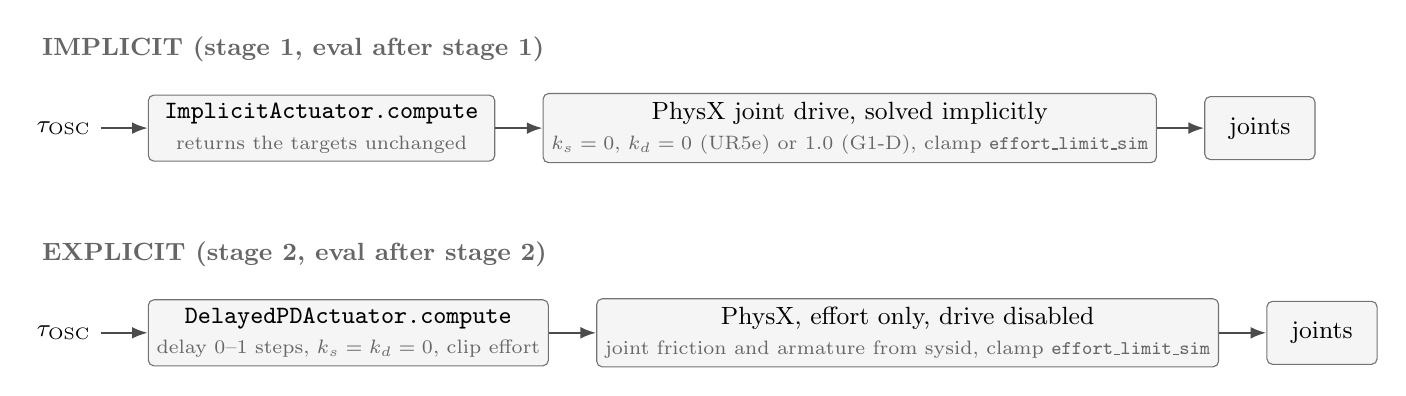
\begin{tikzpicture}[node distance=3mm and 6mm]
  \node[font=\small\bfseries\color{black!60}, anchor=west] at (0,1.0) {IMPLICIT (stage 1, eval after stage 1)};
  \node[font=\small] (t1) at (0.4,0) {$\tau_{\mathrm{OSC}}$};
  \node[blk, right=of t1, minimum width=44mm] (a1) {\code{ImplicitActuator.compute}\\ \subl{returns the targets unchanged}};
  \node[blk, right=of a1, minimum width=62mm] (p1) {PhysX joint drive, solved implicitly\\ \subl{$k_s=0$, $k_d=0$ (UR5e) or $1.0$ (G1-D), clamp \code{effort\_limit\_sim}}};
  \node[blk, right=of p1, minimum width=14mm] (j1) {joints};
  \draw[arr] (t1) -- (a1); \draw[arr] (a1) -- (p1); \draw[arr] (p1) -- (j1);
  \node[font=\small\bfseries\color{black!60}, anchor=west] at (0,-1.6) {EXPLICIT (stage 2, eval after stage 2)};
  \node[font=\small] (t2) at (0.4,-2.6) {$\tau_{\mathrm{OSC}}$};
  \node[blk, right=of t2, minimum width=44mm] (a2) {\code{DelayedPDActuator.compute}\\ \subl{delay 0--1 steps, $k_s=k_d=0$, clip effort}};
  \node[blk, right=of a2, minimum width=62mm] (p2) {PhysX, effort only, drive disabled\\ \subl{joint friction and armature from sysid, clamp \code{effort\_limit\_sim}}};
  \node[blk, right=of p2, minimum width=14mm] (j2) {joints};
  \draw[arr] (t2) -- (a2); \draw[arr] (a2) -- (p2); \draw[arr] (p2) -- (j2);
\end{tikzpicture}}
\myfigcaption{fig:pipes}{The two actuator pipes. In both, the actuator gains are zero and the OSC torque passes through. The explicit pipe adds a delay of zero or one physics step and a software effort clip, and in stage~2 the joints behind it carry the friction and rotor inertia identified on the real arm.}
\end{myfigure}

The configurations below are the two variants for each robot. Note that the G1-D implicit actuator carries a joint damping of $1.0$\,N\,m\,s/rad while every other entry is zero. The reason is the subject of the next section.

\begin{snippetbox}[11]
\snippethead{source/uwlab_assets/uwlab_assets/robots/ur5e_robotiq_gripper/ur5e_robotiq_2f85_gripper.py}{lines 165--175}
\begin{lstlisting}[firstnumber=165]
IMPLICIT_UR5E_ROBOTIQ_2F85 = UR5E_ARTICULATION.copy()  # type: ignore
IMPLICIT_UR5E_ROBOTIQ_2F85.actuators = {
    "arm": ImplicitActuatorCfg(
        joint_names_expr=["shoulder.*", "elbow.*", "wrist.*"],
        stiffness=0.0,
        damping=0.0,
        effort_limit_sim=UR5E_EFFORT_LIMITS,
        velocity_limit_sim=UR5E_VELOCITY_LIMITS,
    ),
    "gripper": ROBOTIQ_2F85.actuators["gripper"],
}
\end{lstlisting}
\end{snippetbox}
\begin{snippetbox}[11]
\snippethead{source/uwlab_assets/uwlab_assets/robots/ur5e_robotiq_gripper/ur5e_robotiq_2f85_gripper.py}{lines 149--163}
\begin{lstlisting}[firstnumber=149]
EXPLICIT_UR5E_ROBOTIQ_2F85 = UR5E_ARTICULATION.copy()  # type: ignore
EXPLICIT_UR5E_ROBOTIQ_2F85.actuators = {
    "arm": DelayedPDActuatorCfg(
        joint_names_expr=["shoulder.*", "elbow.*", "wrist.*"],
        stiffness=0.0,
        damping=0.0,
        effort_limit=UR5E_EFFORT_LIMITS,
        effort_limit_sim=UR5E_EFFORT_LIMITS,
        velocity_limit=UR5E_VELOCITY_LIMITS,
        velocity_limit_sim=UR5E_VELOCITY_LIMITS,
        min_delay=0,
        max_delay=1,
    ),
    "gripper": ROBOTIQ_2F85.actuators["gripper"],
}
\end{lstlisting}
\end{snippetbox}
\begin{snippetbox}[11]
\snippethead{source/uwlab_assets/uwlab_assets/robots/unitree_g1d_dex1/g1d_dex1.py}{lines 137--152}
\begin{lstlisting}[firstnumber=137]
IMPLICIT_G1D_DEX1 = G1D_DEX1_ARTICULATION.copy()  # type: ignore
IMPLICIT_G1D_DEX1.actuators = {
    "arm": ImplicitActuatorCfg(
        joint_names_expr=G1D_ARM_JOINT_REGEX,
        stiffness=0.0,
        # Joint damping lives here (PhysX applies it implicitly, stable at any gain) instead of in the OSC: the
        # wrist links weigh ~85 g (I ~ 5e-4 kg m^2 about the roll axis), and an explicit task-space damping torque
        # of a few N m s/rad at 120 Hz overshoots the velocity each substep and diverges within a handful of
        # substeps (verified with scripts_v2/tools/debug_reset_env-style probes on 2026-10-26). The UR5e gets away
        # with explicit damping only because its wrist links are ~10x heavier.
        damping=1.0,
        effort_limit_sim=G1D_EFFORT_LIMITS,
        velocity_limit_sim=G1D_VELOCITY_LIMITS,
    ),
    "gripper": DEX1_GRIPPER_ACTUATOR,
}
\end{lstlisting}
\end{snippetbox}
\begin{snippetbox}[11]
\snippethead{source/uwlab_assets/uwlab_assets/robots/unitree_g1d_dex1/g1d_dex1.py}{lines 121--135}
\begin{lstlisting}[firstnumber=121]
EXPLICIT_G1D_DEX1 = G1D_DEX1_ARTICULATION.copy()  # type: ignore
EXPLICIT_G1D_DEX1.actuators = {
    "arm": DelayedPDActuatorCfg(
        joint_names_expr=G1D_ARM_JOINT_REGEX,
        stiffness=0.0,
        damping=0.0,
        effort_limit=G1D_EFFORT_LIMITS,
        effort_limit_sim=G1D_EFFORT_LIMITS,
        velocity_limit=G1D_VELOCITY_LIMITS,
        velocity_limit_sim=G1D_VELOCITY_LIMITS,
        min_delay=0,
        max_delay=1,
    ),
    "gripper": DEX1_GRIPPER_ACTUATOR,
}
\end{lstlisting}
\end{snippetbox}

Three small differences remain between the two pipes, and they are worth naming because they are the whole difference between the stage~1 plant and the stage~2 plant as far as the actuator is concerned.
\begin{enumerate}
  \item \textbf{Delay.} The explicit pipe holds each torque for zero or one physics step before it applies. At 120\,Hz that is up to 8.3\,ms, which is the order of the command latency of a real joint controller.
  \item \textbf{Where the effort clamp lives.} The implicit pipe clamps inside the solver with \code{effort\_limit\_sim}. The explicit pipe clamps in Python with \code{effort\_limit} first, and the solver clamp still applies afterwards. The numbers are the same, so the effect is the same.
  \item \textbf{Joint damping on the G1-D.} The implicit G1-D arm has $1.0$\,N\,m\,s/rad of joint damping inside the PhysX drive. The explicit G1-D arm has none. That is a real difference in plant behaviour, and it is discussed in Section~\ref{sec:g1d}.
\end{enumerate}

\subsection{Implicit versus explicit damping, and the light wrist}
\label{sec:stability}

Why does any of this matter if the gains are zero anyway? Because the OSC itself contains a damping term, $K_d\,J\dot q$, and that term is evaluated explicitly: the controller computes it once from the current velocity and holds it for a whole physics step. Consider a single joint with inertia $I$ about its axis and a damping torque $-c\,\omega$ applied this way. Over one step of length $h$ the velocity updates as
\begin{equation}
\begin{aligned}
  \omega_{n+1} &= \Big(1 - \frac{c\,h}{I}\Big)\,\omega_n &&\text{(explicit)},\\
  \omega_{n+1} &= \frac{\omega_n}{1 + c\,h/I} &&\text{(implicit)}.
\end{aligned}
\end{equation}
The implicit update shrinks the velocity for every $c>0$. The explicit update shrinks it only while $c\,h/I < 2$. Beyond that bound each step overshoots zero by more than it started with, and the velocity grows without limit. The bound is therefore
\begin{equation}
  c < \frac{2\,I}{h}.
  \label{eq:bound}
\end{equation}

The numbers for the G1-D wrist are unforgiving. The wrist links weigh about 85\,g, with an inertia of roughly $5\times10^{-4}$\,kg\,m$^2$ about the roll axis, and the physics step is $h = 1/120$\,s. The bound is then about $0.12$\,N\,m\,s/rad. The rotational task-space damping of the OSC is $K_d = 2\zeta\sqrt{K_p}$, which is about $3.5$\,N\,m\,s/rad with the UR5e training gains and about $14$\,N\,m\,s/rad with the evaluation gains. When the wrist roll axis is aligned with the task rotation axis, the transposed Jacobian maps that task damping almost one to one onto the wrist joint. Both values exceed the bound by more than an order of magnitude.

\paragraph{What the code says.} The comment in the G1-D implicit actuator configuration records the empirical version of this argument: an explicit task-space damping torque of a few N\,m\,s/rad at 120\,Hz overshoots the velocity each substep and diverges within a handful of substeps, verified with probe scripts on 26 October 2026. The isolated-link bound of Eq.~\eqref{eq:bound} is a simplification. The effective inertia seen by a joint includes everything downstream of it, and PhysX substeps the solve, so the real threshold is higher than $0.12$. The order of magnitude is what matters, and it explains why the UR5e, whose wrist links are about ten times heavier and carry a 0.5\,kg gripper, tolerates the same damping that destabilises the G1-D.

The G1-D configuration therefore makes two linked choices. The OSC damping ratio is set to zero on all six axes, so the controller applies no explicit damping at all. The damping is moved into the implicit actuator as a joint damping of $1.0$\,N\,m\,s/rad, which PhysX integrates implicitly and which is stable regardless of its value. The gains are otherwise identical to the UR5e recipe.

\begin{snippetbox}[11]
\snippethead{source/uwlab_tasks/uwlab_tasks/manager_based/manipulation/omnireset/config/g1d_dex1/actions.py}{lines 27--50}
\begin{lstlisting}[firstnumber=27]
G1D_DEX1_RELATIVE_OSC = RelCartesianOSCActionCfg(
    asset_name="robot",
    joint_names=G1D_ARM_JOINT_NAMES,
    body_name=G1D_EE_BODY_NAME,
    scale_xyz_axisangle=(0.02, 0.02, 0.02, 0.02, 0.02, 0.2),
    motion_stiffness=(200.0, 200.0, 200.0, 3.0, 3.0, 3.0),
    # No explicit task-space damping: it is unstable on the light G1-D wrist links; the damping is provided
    # implicitly by the arm actuator (see IMPLICIT_G1D_DEX1 in uwlab_assets).
    motion_damping_ratio=(0.0, 0.0, 0.0, 0.0, 0.0, 0.0),
    torque_limit=G1D_TORQUE_LIMIT,
    jacobian_fn=G1D_JACOBIAN_FN,
    # 7-DoF arm: hold the default elbow configuration in the null space of the task
    nullspace_stiffness=2.0,
    nullspace_damping_ratio=1.0,
    nullspace_joint_pos=G1D_DEFAULT_ARM_JOINT_POS,
)
"""Pre-train gains. Same task-space gains as the UR5e recipe: the G1 arm is ~5x lighter, so the loop is if
anything faster; the torque clamp is the per-joint motor limit (25 N m, wrists 5 N m)."""

G1D_DEX1_RELATIVE_OSC_EVAL = G1D_DEX1_RELATIVE_OSC.replace(
    scale_xyz_axisangle=(0.01, 0.01, 0.002, 0.02, 0.02, 0.2),
    motion_stiffness=(1000.0, 1000.0, 1000.0, 50.0, 50.0, 50.0),
    motion_damping_ratio=(1.0, 1.0, 1.0, 1.0, 1.0, 1.0),
)
\end{lstlisting}
\end{snippetbox}

%==============================================================================
\section{Stage 1: Learning the Task}
\label{sec:stage1}

Stage~1 exists to learn the task, not to match the hardware. The simulator is kept as clean as the task allows, so that the policy receives a consistent learning signal while it discovers how to grasp, align and insert. The configuration is the base environment with the training events and the training action set. On the UR5e the robot is the implicit variant throughout the scene definition. On the G1-D the scene also selects the implicit variant, and the environment classes are one-line specialisations of the UR5e ones.

\begin{snippetbox}[11]
\snippethead{source/uwlab_tasks/uwlab_tasks/manager_based/manipulation/omnireset/config/ur5e_robotiq_2f85/rl_state_cfg.py}{lines 728--747}
\begin{lstlisting}[firstnumber=728]
# Training configuration (Stage 1: no curriculum, implicit actuator, no sysid DR)
@configclass
class Ur5eRobotiq2f85RelCartesianOSCTrainCfg(Ur5eRobotiq2f85RlStateCfg):

    events: TrainEventCfg = TrainEventCfg()
    actions: Ur5eRobotiq2f85RelativeOSCAction = Ur5eRobotiq2f85RelativeOSCAction()


# Finetune configuration (Stage 2: explicit actuator, curriculum ramps sysid + gains + scales)
@configclass
class Ur5eRobotiq2f85RelCartesianOSCFinetuneCfg(Ur5eRobotiq2f85RlStateCfg):
    """Finetune config: loads converged Stage 1 policy, explicit actuator from start, curriculum ramps DR."""

    events: FinetuneEventCfg = FinetuneEventCfg()
    actions: Ur5eRobotiq2f85RelativeOSCAction = Ur5eRobotiq2f85RelativeOSCAction()
    curriculum: FinetuneCurriculumsCfg = FinetuneCurriculumsCfg()

    def __post_init__(self):
        super().__post_init__()
        self.scene.robot = EXPLICIT_UR5E_ROBOTIQ_2F85.replace(prim_path="{ENV_REGEX_NS}/Robot")
\end{lstlisting}
\end{snippetbox}
\begin{snippetbox}[11]
\snippethead{source/uwlab_tasks/uwlab_tasks/manager_based/manipulation/omnireset/config/g1d_dex1/rl_state_cfg.py}{lines 202--223}
\begin{lstlisting}[firstnumber=202]
@configclass
class G1dDex1RelCartesianOSCTrainCfg(G1dDex1RlStateCfg):
    """Stage 1 training: implicit actuator, soft gains, four reset-state distributions."""

    events: G1dTrainEventCfg = G1dTrainEventCfg()
    actions: G1dDex1RelativeOSCAction = G1dDex1RelativeOSCAction()


@configclass
class G1dDex1RelCartesianOSCEvalCfg(G1dDex1RlStateCfg):
    """Evaluation after stage 1: ObjectAnywhereEEAnywhere resets only."""

    events: G1dTrainEvalEventCfg = G1dTrainEvalEventCfg()
    actions: G1dDex1RelativeOSCAction = G1dDex1RelativeOSCAction()


@configclass
class G1dDex1RelCartesianOSCStiffEvalCfg(G1dDex1RlStateCfg):
    """Evaluation with the stiff (end-of-curriculum) gains and small action scale."""

    events: G1dTrainEvalEventCfg = G1dTrainEvalEventCfg()
    actions: G1dDex1RelativeOSCEvalAction = G1dDex1RelativeOSCEvalAction()
\end{lstlisting}
\end{snippetbox}

\subsection{What is randomised, and what is not}

The training events are the shared base events plus the reset-state sampler. The base events randomise the things that belong to the \emph{task}: the friction of the robot, the peg, the hole and the table, the masses of the same bodies, and the gripper actuator gains. They deliberately exclude the things that belong to the \emph{motor}: the arm's joint friction, armature and delay, and the OSC gains. The docstring of the base event class says so explicitly, and the training event class only adds the reset sampler.

\begin{snippetbox}[11]
\snippethead{source/uwlab_tasks/uwlab_tasks/manager_based/manipulation/omnireset/config/ur5e_robotiq_2f85/rl_state_cfg.py}{lines 237--255}
\begin{lstlisting}[firstnumber=237]
@configclass
class TrainEventCfg(BaseEventCfg):
    """Training events: material/mass randomization + 4-path resets. No sysid or OSC gain randomization."""

    reset_from_reset_states = EventTerm(
        func=task_mdp.MultiResetManager,
        mode="reset",
        params={
            "dataset_dir": f"{UWLAB_CLOUD_ASSETS_DIR}/Datasets/OmniReset_isaaclab3",
            "reset_types": [
                "ObjectAnywhereEEAnywhere",
                "ObjectRestingEEGrasped",
                "ObjectAnywhereEEGrasped",
                "ObjectPartiallyAssembledEEGrasped",
            ],
            "probs": [0.25, 0.25, 0.25, 0.25],
            "success": "env.reward_manager.get_term_cfg('progress_context').func.success",
        },
    )
\end{lstlisting}
\end{snippetbox}

The reset sampler draws each episode's starting state from one of four pre-recorded distributions with equal probability. These range from ``object anywhere, end effector anywhere'' to ``object partially assembled, end effector grasping'', so the policy practises every phase of the insertion from the first iteration. The reset-state tutorial in this folder describes how those datasets are produced.

\subsection{The controller settings}

The action set is the soft one. The translational stiffness is 200\,N/m, the rotational stiffness 3\,N\,m/rad, and one unit of policy output moves the target by 2\,cm or by 0.02\,rad about $x$ and $y$ and 0.2\,rad about $z$. The UR5e uses a damping ratio of 3 on translation, which is strongly overdamped, and 1 on rotation. The G1-D uses zero for the reason given in Section~\ref{sec:stability}.

\begin{snippetbox}[11]
\snippethead{source/uwlab_tasks/uwlab_tasks/manager_based/manipulation/omnireset/config/ur5e_robotiq_2f85/actions.py}{lines 15--33}
\begin{lstlisting}[firstnumber=15]
UR5E_ROBOTIQ_2F85_RELATIVE_OSC = RelCartesianOSCActionCfg(
    asset_name="robot",
    joint_names=["shoulder.*", "elbow.*", "wrist.*"],
    body_name="wrist_3_link",
    scale_xyz_axisangle=(0.02, 0.02, 0.02, 0.02, 0.02, 0.2),
    motion_stiffness=(200.0, 200.0, 200.0, 3.0, 3.0, 3.0),
    motion_damping_ratio=(3.0, 3.0, 3.0, 1.0, 1.0, 1.0),
    torque_limit=(150.0, 150.0, 150.0, 28.0, 28.0, 28.0),
)

# Eval / sim2real gains (high Kp matched to sysid friction, end-of-curriculum values)
UR5E_ROBOTIQ_2F85_RELATIVE_OSC_EVAL = RelCartesianOSCActionCfg(
    asset_name="robot",
    joint_names=["shoulder.*", "elbow.*", "wrist.*"],
    body_name="wrist_3_link",
    scale_xyz_axisangle=(0.01, 0.01, 0.002, 0.02, 0.02, 0.2),
    motion_stiffness=(1000.0, 1000.0, 1000.0, 50.0, 50.0, 50.0),
    motion_damping_ratio=(1.0, 1.0, 1.0, 1.0, 1.0, 1.0),
    torque_limit=(150.0, 150.0, 150.0, 28.0, 28.0, 28.0),
\end{lstlisting}
\end{snippetbox}

Inside the action term these numbers become per-environment tensors. The per-environment copy is what allows the stage~2 events to change the gains of each environment independently without touching the configuration.

\begin{snippetbox}[11]
\snippethead{source/uwlab_tasks/uwlab_tasks/manager_based/manipulation/omnireset/mdp/actions/task_space_actions.py}{lines 64--73, 94--95}
\begin{lstlisting}[firstnumber=64]
# Controller gains (per-env for domain randomization): Kd = 2 * sqrt(Kp) * damping_ratio
kp = torch.tensor(cfg.motion_stiffness, device=self.device, dtype=torch.float32)
damping_ratio = torch.tensor(cfg.motion_damping_ratio, device=self.device, dtype=torch.float32)
kd = 2.0 * torch.sqrt(kp) * damping_ratio
# Store defaults (1D) and expand to per-env (N, 6)
self._kp_default = kp
self._kd_default = kd
self._damping_ratio_default = damping_ratio
self._kp = kp.unsqueeze(0).expand(self.num_envs, -1).clone()
self._kd = kd.unsqueeze(0).expand(self.num_envs, -1).clone()
\end{lstlisting}
\snippetelide
\begin{lstlisting}[firstnumber=94]
# Action scaling
self._scale = torch.tensor(cfg.scale_xyz_axisangle, device=self.device, dtype=torch.float32)
\end{lstlisting}
\end{snippetbox}

\subsection{The learner}

The learner is proximal policy optimisation (PPO)~\cite{schulman2017ppo} from RSL-RL~\cite{rudin2022walk}. Table~\ref{tab:ppo} lists the settings that matter for reading the curriculum timings later. The G1-D runner inherits all of them and changes only the experiment name.

\begin{mytable}
\mytabcaption{tab:ppo}{PPO runner settings shared by both robots.}
{\small
\begin{tabular}{@{}p{0.26\linewidth}p{0.24\linewidth}p{0.44\linewidth}@{}}
\toprule Setting & Value & Meaning\\\midrule
policy rate & 10\,Hz & decimation 12 at a physics step of $1/120$\,s\\
rollout length & 32 steps per env & one PPO iteration is 32 policy steps, or 3.2\,s of simulated time per environment\\
learning rate & $10^{-4}$, adaptive & adjusted to hold a KL divergence of 0.01 between updates\\
discount, GAE & 0.99, 0.95 & horizon of about 100 policy steps\\
entropy coefficient & 0.006 & exploration bonus\\
network & MLP 512, 256, 128, 64, ELU & actor and critic, with observation normalisation\\
action distribution & heteroscedastic Gaussian & state-dependent log standard deviation in $[0.001, 2]$\\
\bottomrule
\end{tabular}}
\end{mytable}

\begin{snippetbox}[11]
\snippethead{source/uwlab_tasks/uwlab_tasks/manager_based/manipulation/omnireset/config/ur5e_robotiq_2f85/agents/rsl_rl_cfg.py}{lines 17--24, 47--60}
\begin{lstlisting}[firstnumber=17]
@configclass
class Base_PPORunnerCfg(RslRlOnPolicyRunnerCfg):
    num_steps_per_env = 32
    max_iterations = 40000
    save_interval = 100
    obs_groups = {"actor": ["policy"], "critic": ["policy"]}
    resume = False
    experiment_name = "ur5e_robotiq_2f85_omnireset_agent"
\end{lstlisting}
\snippetelide
\begin{lstlisting}[firstnumber=47]
    algorithm = RslRlPpoAlgorithmCfg(
        value_loss_coef=1.0,
        use_clipped_value_loss=True,
        normalize_advantage_per_mini_batch=False,
        clip_param=0.2,
        entropy_coef=0.006,
        num_learning_epochs=5,
        num_mini_batches=4,
        learning_rate=1.0e-4,
        schedule="adaptive",
        gamma=0.99,
        lam=0.95,
        desired_kl=0.01,
        max_grad_norm=1.0,
\end{lstlisting}
\end{snippetbox}

%==============================================================================
\section{Stage 2: Moving the Policy Toward the Real Robot}
\label{sec:stage2}

A policy that has converged in stage~1 has never felt joint friction, has never waited for a delayed torque, and has only ever pushed with soft gains and large steps. Each of these is different on the hardware. Stage~2 closes the gap by continuing training while the simulator is moved, a little at a time, from the stage~1 plant to the real one. It is a fine-tuning stage because it starts from the stage~1 checkpoint rather than from random weights.

\subsection{The configuration}

The fine-tune environment differs from the training environment in three declarations. The events are the fine-tune events, which add two randomisation terms. The curriculum is no longer empty. And after the base initialisation, the scene's robot is replaced by the explicit variant, so the delayed actuator is in place from the first step of stage~2. The listing of the two environment classes in Section~\ref{sec:stage1} shows all three.

The stage~1 checkpoint is loaded through the training script's resume mechanism. Passing a checkpoint path makes the runner load the weights before the first iteration, and training then continues under the fine-tune environment.

\begin{snippetbox}[11]
\snippethead{scripts/reinforcement_learning/rsl_rl/train.py}{lines 179--184, 210--214}
\begin{lstlisting}[firstnumber=179]
# save resume path before creating a new log_dir
if args_cli.resume_path is not None:
    resume_path = retrieve_file_path(args_cli.resume_path)
    agent_cfg.resume = True
elif agent_cfg.resume or agent_cfg.algorithm.class_name == "Distillation":
    resume_path = get_checkpoint_path(log_root_path, agent_cfg.load_run, agent_cfg.load_checkpoint)
\end{lstlisting}
\snippetelide
\begin{lstlisting}[firstnumber=210]
# load the checkpoint
if agent_cfg.resume or agent_cfg.algorithm.class_name == "Distillation":
    print(f"[INFO]: Loading model checkpoint from: {resume_path}")
    # load previously trained model
    runner.load(resume_path)
\end{lstlisting}
\end{snippetbox}

\subsection{The progress variable and what it controls}

Everything that stage~2 changes about the simulator is driven by a scalar progress variable $p\in[0,1]$. At $p=0$ the simulator is the stage~1 simulator with the explicit actuator. At $p=1$ it is the evaluation simulator. The progress variable is stored on the event terms and read every time they run, which is at every environment reset. Three families of quantities depend on it.

\paragraph{Arm dynamics from system identification.} The calibrated armature $a^{\mathrm{id}}_j$, static friction $\mu^{\mathrm{id}}_{s,j}$, dynamic-to-static ratio $\rho^{\mathrm{id}}_j$ and viscous friction $b^{\mathrm{id}}_j$ of each joint $j$ are read from the robot's metadata file~\cite{bjelonic2025pace}. At each reset of an environment, a fresh scale $s\sim U(0.8,1.2)$ is drawn per joint and per quantity, and the values written into PhysX are
\begin{equation}
\begin{aligned}
  a_j &= (1-p)\,a^{0}_j + p\,s\,a^{\mathrm{id}}_j,\\
  \mu_{s,j} &= p\,s\,\mu^{\mathrm{id}}_{s,j}, \qquad
  \mu_{d,j} = \min\!\big(s\,\rho^{\mathrm{id}}_j\,\mu_{s,j},\;\mu_{s,j}\big),\\
  b_j &= p\,s\,b^{\mathrm{id}}_j,\\
  d &\sim U\{0,\dots,\mathrm{round}(p\,d_{\max})\}, \quad d_{\max}=1,
\end{aligned}
\end{equation}
where $a^{0}_j$ is the armature the asset started with and $d$ is the motor delay in physics steps. Friction starts at exactly zero and the delay starts at exactly zero, so the $p=0$ plant is frictionless and instantaneous, as in stage~1.

\begin{snippetbox}[11]
\snippethead{source/uwlab_tasks/uwlab_tasks/manager_based/manipulation/omnireset/mdp/events.py}{lines 1701--1734}
\begin{lstlisting}[firstnumber=1701]
p = self.scale_progress

def _scale(nominal):
    val = torch.as_tensor(nominal, device=device, dtype=torch.float32)
    return val * (lo + torch.rand(N, n_joints, device=device) * (hi - lo))

# Armature and friction: interpolate from the startup model to sysid
if self._initial_armature is None:
    self._initial_armature = self.robot.data.joint_armature.torch[:, self.joint_ids].clone()
arm_vals = self._initial_armature[env_ids] * (1.0 - p) + _scale(self.armature) * p
sfric_vals = _scale(self.static_friction) * p
dratio_vals = _scale(self.dynamic_ratio) * p
dfric_vals = torch.minimum(dratio_vals * sfric_vals, sfric_vals)
vfric_vals = _scale(self.viscous_friction) * p

self.robot.write_joint_armature_to_sim_index(armature=arm_vals, joint_ids=self.joint_ids, env_ids=env_ids)
self.robot.write_joint_friction_coefficient_to_sim_index(
    joint_friction_coeff=sfric_vals,
    joint_dynamic_friction_coeff=dfric_vals,
    joint_viscous_friction_coeff=vfric_vals,
    joint_ids=self.joint_ids,
    env_ids=env_ids,
)

# Motor delay scaled by ADR progress (if actuator supports it)
delay_lo, delay_hi = delay_range
actuator = self.robot.actuators[self.actuator_name]
if hasattr(actuator, "positions_delay_buffer"):
    effective_hi = int(round(p * delay_hi))
    effective_lo = min(delay_lo, effective_hi)
    delays = torch.randint(effective_lo, effective_hi + 1, (N,), device=device, dtype=torch.int)
    actuator.positions_delay_buffer.set_time_lag(delays, env_ids)
    actuator.velocities_delay_buffer.set_time_lag(delays, env_ids)
    actuator.efforts_delay_buffer.set_time_lag(delays, env_ids)
\end{lstlisting}
\end{snippetbox}

\paragraph{Controller gains.} The same event mechanism moves the OSC gains of each environment from the soft training values $K_p^0,\zeta^0$ toward randomised copies of the terminal values $K_p^1,\zeta^1$. Separate scales are drawn for the translational and rotational blocks and for stiffness and damping ratio, so four scalars per environment in total:
\begin{equation}
\begin{aligned}
  K_p(p) &= K_p^0 + p\,\big(s\,K_p^1 - K_p^0\big),\\
  \zeta(p) &= \zeta^0 + p\,\big(s'\,\zeta^1 - \zeta^0\big),\\
  K_d &= 2\,\zeta(p)\sqrt{K_p(p)}.
\end{aligned}
\end{equation}

\begin{snippetbox}[11]
\snippethead{source/uwlab_tasks/uwlab_tasks/manager_based/manipulation/omnireset/mdp/events.py}{lines 1862--1867, 1872--1888, 1898--1899}
\begin{lstlisting}[firstnumber=1862]
p = self.scale_progress

s_xyz = lo + torch.rand(n, 1, device=env.device) * (hi - lo)
s_rpy = lo + torch.rand(n, 1, device=env.device) * (hi - lo)
s_dr_xyz = lo + torch.rand(n, 1, device=env.device) * (hi - lo)
s_dr_rpy = lo + torch.rand(n, 1, device=env.device) * (hi - lo)
\end{lstlisting}
\snippetelide
\begin{lstlisting}[firstnumber=1872]
if terminal_kp is not None and terminal_damping_ratio is not None:
    # Terminal Kp with randomization
    kp_term = torch.tensor(terminal_kp, device=env.device, dtype=torch.float32)
    target_kp = kp_term.unsqueeze(0).repeat(n, 1)
    target_kp[:, :3] *= s_xyz
    target_kp[:, 3:] *= s_rpy

    dr_term = torch.tensor(terminal_damping_ratio, device=env.device, dtype=torch.float32)
    target_dr = dr_term.unsqueeze(0).repeat(n, 1)
    target_dr[:, :3] *= s_dr_xyz
    target_dr[:, 3:] *= s_dr_rpy

    # Interpolate from action defaults (initial) to terminal
    init_kp = kp_default.unsqueeze(0)
    init_dr = dr_default.unsqueeze(0)
    new_kp = init_kp + p * (target_kp - init_kp)
    new_dr = init_dr + p * (target_dr - init_dr)
\end{lstlisting}
\snippetelide
\begin{lstlisting}[firstnumber=1898]
self._action_term._kp[env_ids] = new_kp
self._action_term._kd[env_ids] = 2.0 * torch.sqrt(new_kp) * new_dr
\end{lstlisting}
\end{snippetbox}

\paragraph{Action scale.} The per-step displacement that one unit of policy output commands shrinks linearly from the training scale $\sigma^0$ to the terminal scale $\sigma^1$. This one is applied to the action term directly and is shared by all environments:
\begin{equation}
\begin{aligned}
  \sigma(p) &= \sigma^0 + p\,\big(\sigma^1 - \sigma^0\big),\\
  \sigma^0 &= (2,2,2)\,\mathrm{cm}, \qquad \sigma^1 = (1,1,0.2)\,\mathrm{cm}.
\end{aligned}
\end{equation}

\begin{snippetbox}[11]
\snippethead{source/uwlab_tasks/uwlab_tasks/manager_based/manipulation/omnireset/mdp/events.py}{lines 2084--2096}
\begin{lstlisting}[firstnumber=2084]
success_rates = self._reset_term.success_monitor.get_success_rate()
mean_success = success_rates.mean().item()

if mean_success > success_threshold_up:
    self._progress = min(1.0, self._progress + delta)
elif mean_success < success_threshold_down:
    self._progress = max(0.0, self._progress - delta)

initial = torch.tensor(initial_scales, device=env.device, dtype=torch.float32)
target = torch.tensor(target_scales, device=env.device, dtype=torch.float32)
effective = initial + self._progress * (target - initial)

self._action_term._scale = effective
\end{lstlisting}
\end{snippetbox}

The fine-tune events and the terminal values are declared together. The curriculum class names the event terms it drives and sets the thresholds of the update rule.

\begin{snippetbox}[11]
\snippethead{source/uwlab_tasks/uwlab_tasks/manager_based/manipulation/omnireset/config/ur5e_robotiq_2f85/rl_state_cfg.py}{lines 318--352}
\begin{lstlisting}[firstnumber=318]
@configclass
class FinetuneEventCfg(TrainEventCfg):
    """Finetune events: curriculum-ramped sysid + OSC gains + 4-path resets. Explicit actuator from start."""

    randomize_arm_sysid = EventTerm(
        func=task_mdp.randomize_arm_from_sysid,
        mode="reset",
        params={
            "asset_cfg": SceneEntityCfg("robot"),
            "joint_names": [
                "shoulder_pan_joint",
                "shoulder_lift_joint",
                "elbow_joint",
                "wrist_1_joint",
                "wrist_2_joint",
                "wrist_3_joint",
            ],
            "actuator_name": "arm",
            "scale_range": (0.8, 1.2),
            "delay_range": (0, 1),
            "initial_scale_progress": 0.0,
        },
    )

    randomize_osc_gains = EventTerm(
        func=task_mdp.randomize_rel_cartesian_osc_gains,
        mode="reset",
        params={
            "action_name": "arm",
            "scale_range": (0.8, 1.2),
            "terminal_kp": (1000.0, 1000.0, 1000.0, 50.0, 50.0, 50.0),
            "terminal_damping_ratio": (1.0, 1.0, 1.0, 1.0, 1.0, 1.0),
            "initial_scale_progress": 0.0,
        },
    )
\end{lstlisting}
\end{snippetbox}
\begin{snippetbox}[11]
\snippethead{source/uwlab_tasks/uwlab_tasks/manager_based/manipulation/omnireset/config/ur5e_robotiq_2f85/rl_state_cfg.py}{lines 578--610}
\begin{lstlisting}[firstnumber=578]
@configclass
class FinetuneCurriculumsCfg:
    """Finetune curriculum: ADR sysid + action scale ramp. No actuator swap (explicit from start)."""

    adr_sysid = CurrTerm(
        func=task_mdp.adr_sysid_curriculum,
        params={
            "event_term_names": ["randomize_arm_sysid", "randomize_osc_gains"],
            "reset_event_name": "reset_from_reset_states",
            "success_threshold_up": 0.95,
            "success_threshold_down": 0.9,
            "delta": 0.01,
            "update_every_n_steps": 200,
            "initial_scale_progress": 0.0,
            "warmup_success_threshold": 0.95,
        },
    )

    action_scale = CurrTerm(
        func=task_mdp.action_scale_curriculum,
        params={
            "action_name": "arm",
            "reset_event_name": "reset_from_reset_states",
            "initial_scales": [0.02, 0.02, 0.02, 0.02, 0.02, 0.2],
            "target_scales": [0.01, 0.01, 0.002, 0.02, 0.02, 0.2],
            "success_threshold_up": 0.95,
            "success_threshold_down": 0.9,
            "delta": 0.01,
            "update_every_n_steps": 200,
            "initial_progress": 0.0,
        },
    )

\end{lstlisting}
\end{snippetbox}

\subsection{The update rule}

The progress variable is not advanced on a timer. It is advanced by the policy's own success rate, so the simulator only becomes harder when the policy has shown that it can cope with the current difficulty. The rule is a simple hysteresis controller. Let $\bar s$ be the mean success rate across the reset-state distributions, as reported by the reset sampler's success monitor. Every 200 environment steps,
\begin{equation}
  p \leftarrow
  \begin{cases}
    \min(1,\;p+0.01) & \text{if } \bar s > 0.95,\\
    \max(0,\;p-0.01) & \text{if } \bar s < 0.90,\\
    p & \text{otherwise.}
  \end{cases}
  \label{eq:rule}
\end{equation}
The band between 0.90 and 0.95 is where the policy is allowed to recover without the difficulty changing. A separate warm-up gate holds $p=0$ until the success rate has reached 0.95 at least once, so that a freshly loaded checkpoint which performs poorly under the new actuator is given time before anything else changes. Once opened, the gate stays open.

\begin{snippetbox}[11]
\snippethead{source/uwlab_tasks/uwlab_tasks/manager_based/manipulation/omnireset/mdp/events.py}{lines 1977--1980, 1988--1989, 1991--1994, 2002--2011}
\begin{lstlisting}[firstnumber=1977]
# Only update once every N env steps (agnostic to num_envs)
current_step = env.common_step_counter
if (current_step - self._last_update_step) < update_every_n_steps:
    return self._last_state
\end{lstlisting}
\snippetelide
\begin{lstlisting}[firstnumber=1988]
success_rates = self._reset_term.success_monitor.get_success_rate()
mean_success = success_rates.mean().item()
\end{lstlisting}
\snippetelide
\begin{lstlisting}[firstnumber=1991]
# Warmup gate: hold scale_progress until success exceeds threshold
if not self._warmed_up:
    if mean_success >= self._warmup_threshold:
        self._warmed_up = True
\end{lstlisting}
\snippetelide
\begin{lstlisting}[firstnumber=2002]
# Update scale_progress based on thresholds
current_progress = self._event_terms[0].scale_progress if self._event_terms else 0.0
if mean_success > success_threshold_up:
    current_progress = min(1.0, current_progress + delta)
elif mean_success < success_threshold_down:
    current_progress = max(0.0, current_progress - delta)

# Apply to all target event terms
for term in self._event_terms:
    term.scale_progress = current_progress
\end{lstlisting}
\end{snippetbox}

There are two independent copies of this rule. One drives the arm dynamics and the OSC gains together, so a single progress value moves friction, delay and gains in lockstep. The other drives the action scale. Both read the same success rate and use the same thresholds and step, but each keeps its own counter and its own progress, so in practice they drift apart by a few hundredths. Figure~\ref{fig:curriculum} shows a schematic run of the rule.

\begin{myfigure}
\begin{tikzpicture}
\begin{groupplot}[group style={group size=1 by 2, vertical sep=6mm}, width=0.9\linewidth, height=0.27\linewidth,
  xmin=0, xmax=1000, grid=none, tick label style={font=\scriptsize}, label style={font=\scriptsize},
  axis line style={black!40}, every axis plot/.append style={line width=1.2pt}, clip=false]
\nextgroupplot[ymin=0.5, ymax=1.02, ytick={0.5,0.75,1.0}, ylabel={mean success (schematic)}, xticklabels={}, legend style={font=\scriptsize, draw=none, at={(0.98,0.08)}, anchor=south east}]
  \addplot[series1] table[x=it, y=success] {curriculum.dat}; \addlegendentry{mean success rate}
  \draw[black!50, dashed] (axis cs:0,0.95) -- (axis cs:1000,0.95) node[pos=1, anchor=south east, font=\tiny\color{black!60}] {raise above 0.95};
  \draw[black!50, dashed] (axis cs:0,0.90) -- (axis cs:1000,0.90) node[pos=1, anchor=north east, font=\tiny\color{black!60}] {lower below 0.90};
\nextgroupplot[ymin=0, ymax=1.05, ytick={0,0.5,1}, ylabel={progress $p$}, xlabel={PPO iteration (32 policy steps each)}, legend style={font=\scriptsize, draw=none, at={(0.98,0.08)}, anchor=south east}]
  \addplot[series2] table[x=it, y=p] {curriculum.dat}; \addlegendentry{curriculum progress $p$}
  \draw[black!50, dashed] (axis cs:190,0) -- (axis cs:190,1.05) node[pos=0.1, anchor=west, font=\tiny\color{black!60}] {warm-up gate opens};
\end{groupplot}
\end{tikzpicture}
\myfigcaption{fig:curriculum}{A schematic run of the update rule, produced by a toy model and not by a training log. The success rate rises as the policy learns, the warm-up gate opens when it first touches 0.95, and progress then climbs in steps of 0.01 whenever success stays above the upper threshold. Around the middle of the ramp the plant becomes noticeably harder, success falls below 0.90, progress retreats until the policy recovers, and the climb resumes. The ramp ends when progress reaches 1.}
\end{myfigure}

The timings follow from the numbers in Eq.~\eqref{eq:rule}. The counter is the environment's global step counter, which advances once per policy step regardless of how many parallel environments there are. Reaching $p=1$ from 0 needs at least 100 raises, hence at least 20\,000 policy steps. At 32 policy steps per PPO iteration, that is at least 625 iterations, or 2\,000\,s of simulated time per environment. Any excursion below 0.90 adds to this, because every retreat has to be climbed again.

\subsection{Why ramp rather than switch}

One might ask why the plant is not simply switched to its final form at the start of stage~2. The reason is that the stage~1 policy is tuned to the stage~1 plant. Under stiff gains and real friction the same actions produce different motion, the observations drift out of the distribution the policy has seen, and the success rate collapses. PPO can recover from a collapse, but it does so slowly and sometimes to a worse policy. The ramp keeps the policy inside a regime where it mostly succeeds, so every update is made from informative, mostly successful rollouts. The success gate turns the ramp speed into a measured quantity rather than a guess.

%==============================================================================
\section{The Evaluation Environments}
\label{sec:eval}

There are two evaluation environments per robot, one per stage, and each reproduces the plant of the stage it evaluates. The evaluation after stage~1 uses the implicit actuator and the soft action set. The evaluation after stage~2 uses the explicit actuator, the stiff action set, and the fixed variants of the two stage~2 events. Both reduce the reset distribution to the single ``object anywhere, end effector anywhere'' case.

\begin{snippetbox}[11]
\snippethead{source/uwlab_tasks/uwlab_tasks/manager_based/manipulation/omnireset/config/ur5e_robotiq_2f85/rl_state_cfg.py}{lines 750--769}
\begin{lstlisting}[firstnumber=750]
# Evaluation configuration (after Stage 1: implicit actuator, soft gains, no sysid DR)
@configclass
class Ur5eRobotiq2f85RelCartesianOSCEvalCfg(Ur5eRobotiq2f85RlStateCfg):
    """Eval after Stage 1: implicit actuator, soft gains, large action scale, no sysid DR."""

    events: TrainEvalEventCfg = TrainEvalEventCfg()
    actions: Ur5eRobotiq2f85RelativeOSCAction = Ur5eRobotiq2f85RelativeOSCAction()


# Evaluation configuration (after Stage 2: explicit actuator, stiff gains, fixed sysid)
@configclass
class Ur5eRobotiq2f85RelCartesianOSCFinetuneEvalCfg(Ur5eRobotiq2f85RlStateCfg):
    """Eval after Stage 2: explicit actuator, stiff gains, small action scale, fixed sysid + OSC gains."""

    events: FinetuneEvalEventCfg = FinetuneEvalEventCfg()
    actions: Ur5eRobotiq2f85RelativeOSCEvalAction = Ur5eRobotiq2f85RelativeOSCEvalAction()

    def __post_init__(self):
        super().__post_init__()
        self.scene.robot = EXPLICIT_UR5E_ROBOTIQ_2F85.replace(prim_path="{ENV_REGEX_NS}/Robot")
\end{lstlisting}
\end{snippetbox}

The fixed event variants are subclasses of the stage~2 events that pin $p=1$ and skip the curriculum. They still draw the $U(0.8,1.2)$ scales at every reset, so the stage~2 evaluation sees the same spread of plants that the end of training saw, rather than one nominal plant. The stiff action set supplies the terminal gains and scale as the defaults that those scales multiply.

\begin{snippetbox}[11]
\snippethead{source/uwlab_tasks/uwlab_tasks/manager_based/manipulation/omnireset/config/ur5e_robotiq_2f85/rl_state_cfg.py}{lines 274--304}
\begin{lstlisting}[firstnumber=274]
@configclass
class FinetuneEvalEventCfg(BaseEventCfg):
    """Eval after Stage 2: fixed sysid + OSC gains (scale_progress=1) + 1-path resets."""

    randomize_arm_sysid = EventTerm(
        func=task_mdp.randomize_arm_from_sysid_fixed,
        mode="reset",
        params={
            "asset_cfg": SceneEntityCfg("robot"),
            "joint_names": [
                "shoulder_pan_joint",
                "shoulder_lift_joint",
                "elbow_joint",
                "wrist_1_joint",
                "wrist_2_joint",
                "wrist_3_joint",
            ],
            "actuator_name": "arm",
            "scale_range": (0.8, 1.2),
            "delay_range": (0, 1),
        },
    )

    randomize_osc_gains = EventTerm(
        func=task_mdp.randomize_rel_cartesian_osc_gains_fixed,
        mode="reset",
        params={
            "action_name": "arm",
            "scale_range": (0.8, 1.2),
        },
    )
\end{lstlisting}
\end{snippetbox}

%==============================================================================
\section{Why Training and Evaluation Differ}
\label{sec:why}

Table~\ref{tab:settings} showed three controller parameters that differ between the training and evaluation action sets: the stiffness, the damping ratio and the action scale. None of them is a separate design. The evaluation values are the end of the stage~2 ramp, and the training values are its start. The question is therefore why the ramp exists at all, parameter by parameter.

\subsection{Stiffness: friction sets a floor on the useful gain}

Consider the controller holding the end effector against a resisting force. At rest the task-space PD law reduces to $F = K_p\,e$, so a resisting force $F_f$ that the controller must overcome leaves a steady-state error
\begin{equation}
  e_{\mathrm{ss}} = \frac{F_f}{K_p}.
\end{equation}
On the real arm, joint friction and the stiction of a peg in a hole both act as such a force. Suppose the friction of the wrist joints is equivalent to 5\,N at the end effector, which is an illustrative figure rather than a measurement. At $K_p = 200$\,N/m the controller stops 25\,mm short of its target. At $K_p = 1000$\,N/m it stops 5\,mm short. For a peg with a fraction of a millimetre of clearance, the first number makes the task impossible and the second makes it merely hard. The stiff gain is the one that the real robot's controller runs, chosen against the friction found by system identification. The soft gain exists only because it is easier to learn under, as Section~\ref{sec:whynot} explains.

\subsection{Damping ratio: overdamped for exploration, critical for deployment}

The UR5e trains with a translational damping ratio of 3, which is strongly overdamped. An overdamped loop approaches its target slowly and never overshoots, so a random early policy cannot make the arm swing through the table or the hole. The evaluation ratio of 1 is critically damped, which is the fastest response without overshoot, and is what the hardware controller uses. The G1-D trains with no explicit damping at all, for the stability reason in Section~\ref{sec:stability}, which makes its jump from training to evaluation damping larger than the UR5e's.

\subsection{Action scale: how far the arm moves per policy step}

With soft gains the controller only ever reaches a fraction of a 2\,cm step within the 0.1\,s policy period, so the effective motion is gentle even though the commanded step is large. With stiff gains the step is reached within the period, and the step size becomes the speed:
\begin{equation}
  v = \frac{\sigma}{\Delta t_{\mathrm{policy}}} =
  \begin{cases}
    0.2\,\mathrm{m/s} & \text{at } \sigma = 2\,\mathrm{cm},\\
    0.1\,\mathrm{m/s} & \text{at } \sigma = 1\,\mathrm{cm},\\
    0.02\,\mathrm{m/s} & \text{at } \sigma = 2\,\mathrm{mm}.
  \end{cases}
\end{equation}
Shrinking the scale as the gains stiffen keeps the end-effector speed in a range that insertion tolerates, and the 2\,mm vertical scale gives the policy millimetre control over the one axis that needs it. The alternative of clipping the pose error inside the controller would saturate the PD law and flatten the relationship between action and motion. Scaling the action instead keeps that relationship linear, which is what a policy gradient needs.

\subsection{Why not train stiff from the start}
\label{sec:whynot}

Put the three together and the ordering is forced. A stiff controller with a 2\,cm step applies a 20\,N task force to every step, against 4\,N for the soft one. An untrained policy emits random 2\,cm steps ten times a second. Stiff gains therefore mean hard contacts, frequent collisions and many episodes that end in a termination before any reward is collected. Soft gains make exploration survivable. Once the policy knows what to do, the gains can be raised and the steps shortened, and the policy adapts to the changed response because it observes the end-effector pose and velocity rather than its own commands.

%==============================================================================
\section{The G1-D Today}
\label{sec:g1d}

The G1-D configuration implements stage~1 and its evaluation. It does not yet implement stage~2. Table~\ref{tab:classes} lists what exists for each robot.

\begin{mytable}
\mytabcaption{tab:classes}{Environment classes per robot.}
{\scriptsize
\begin{tabular}{@{}p{0.17\linewidth}p{0.4\linewidth}p{0.36\linewidth}@{}}
\toprule Role & UR5e + Robotiq 2F-85 & G1-D + Dex1-1\\\midrule
stage 1 train & \code{Ur5eRobotiq2f85\allowbreak RelCartesianOSC\allowbreak TrainCfg} & \code{G1dDex1\allowbreak RelCartesianOSC\allowbreak TrainCfg}\\
eval after stage 1 & \code{Ur5eRobotiq2f85\allowbreak RelCartesianOSC\allowbreak EvalCfg} & \code{G1dDex1\allowbreak RelCartesianOSC\allowbreak EvalCfg}\\
stage 2 fine-tune & \code{Ur5eRobotiq2f85\allowbreak RelCartesianOSC\allowbreak FinetuneCfg} & none\\
eval after stage 2 & \code{Ur5eRobotiq2f85\allowbreak RelCartesianOSC\allowbreak FinetuneEvalCfg} & \code{G1dDex1\allowbreak RelCartesianOSC\allowbreak StiffEvalCfg} (partial, see below)\\
\bottomrule
\end{tabular}}
\end{mytable}

Three observations follow from reading the configuration against the UR5e recipe. They are listed as facts about the current code, not as a plan.
\begin{enumerate}
  \item \textbf{The stiff evaluation evaluates an untrained regime.} The G1-D stiff evaluation config applies the terminal gains and scale to a stage~1 policy, but with the implicit actuator and without the fixed sysid events. A stage~1 policy has trained at $K_p=200$ with $\zeta=0$ and is here evaluated at $K_p=1000$ with $\zeta=1$. A lower success rate than the plain evaluation is expected, and the gap is a measure of how much a stage~2 would change rather than a defect.
  \item \textbf{The explicit G1-D actuator has no joint damping.} The implicit variant carries the $1.0$\,N\,m\,s/rad that replaces the OSC's explicit damping. The explicit variant, which a stage~2 would use, sets damping to zero, and the terminal damping ratio of 1 would re-introduce the explicit task-space damping of about $14$\,N\,m\,s/rad that Section~\ref{sec:stability} argues is unstable on this wrist.
  \item \textbf{There is no system identification for the G1-D.} The sysid event reads an \code{armature}, \code{static\_friction}, \code{dynamic\_ratio} and \code{viscous\_friction} block from the robot's metadata file. The G1-D metadata file has no such block, so the UR5e fine-tune events cannot be instantiated against it as they stand.
\end{enumerate}

%==============================================================================
\section{Where Everything Lives}
\label{sec:files}

All paths are relative to the repository root. The task package root \path{source/uwlab_tasks/uwlab_tasks/manager_based/manipulation/omnireset} is abbreviated to \code{omnireset/}.

\begin{mytable}
\mytabcaption{tab:files}{File index.}
{\scriptsize
\begin{tabular}{@{}p{0.36\linewidth}p{0.6\linewidth}@{}}
\toprule What & Where\\\midrule
implicit, ideal and delayed PD actuators & Isaac Lab 17.0.2, \path{isaaclab/actuators/actuator_pd.py}\\
UR5e articulation, implicit and explicit variants & \path{source/uwlab_assets/uwlab_assets/robots/ur5e_robotiq_gripper/ur5e_robotiq_2f85_gripper.py}\\
G1-D articulation, implicit and explicit variants & \path{source/uwlab_assets/uwlab_assets/robots/unitree_g1d_dex1/g1d_dex1.py}\\
OSC action term, per-environment gains & \path{omnireset/mdp/actions/task_space_actions.py}\\
UR5e action sets, soft and stiff & \path{omnireset/config/ur5e_robotiq_2f85/actions.py}\\
G1-D action sets, soft and stiff & \path{omnireset/config/g1d_dex1/actions.py}\\
UR5e environments, events and curriculum & \path{omnireset/config/ur5e_robotiq_2f85/rl_state_cfg.py}\\
G1-D environments and events & \path{omnireset/config/g1d_dex1/rl_state_cfg.py}\\
sysid, gain and action-scale events, curriculum terms & \path{omnireset/mdp/events.py}\\
PPO runner & \path{omnireset/config/ur5e_robotiq_2f85/agents/rsl_rl_cfg.py}\\
checkpoint loading & \path{scripts/reinforcement_learning/rsl_rl/train.py}, flag \code{--resume\_path}\\
registered task names & \code{OmniReset-\allowbreak Ur5eRobotiq2f85-\allowbreak RelCartesianOSC-\allowbreak State-\allowbreak \{,Finetune-,Play-,Finetune-Play-\}v0}, \code{OmniReset-\allowbreak G1dDex1-\allowbreak RelCartesianOSC-\allowbreak State-\allowbreak \{,Play-\}v0}\\
\bottomrule
\end{tabular}}
\end{mytable}


\bibliography{references}

\end{document}
